\newcommand{\tmp}{TMP36}
\newcommand{\vs}{\texttt{+vs}}
\newcommand{\vout}{\texttt{vout}}
\newcommand{\gnd}{\texttt{gnd}}
\newcommand{\pinV}{\texttt{5v}}
\newcommand{\sensorpin}{\texttt{A0}}
\newcommand{\txtloop}{\texttt{loop}}

\chapter{Misura di Temperature con Arduino}
    Tra le esperienze svolte con Arduino Uno riporto in particolare la misura della variazione della temperatura della mia stanza da letto in seguito all'accensione del riscaldamento in casa.
    \section{L'esperimento}
            L'obiettivo dell'esperienza è quello di valutare qualitativamente l'andamento della temperatura della stanza per fare una stima di quanto velocemente si riscaldi e a quale temperatura tenda asintoticamente.
        \subsection{Preparazione della stanza}
            Per massimizzare l'escursione termica ho effettuato la misura durante una sera invernale avendo preventivamente aperto le finestre per abbassare la temperatura della stanza.
            
            Per migliorare la circolazione dell'aria ed evitare un eccessivo gradiente di temperatura---il radiatore caldo si trova in un angolo della stanza mentre i vetri freddi della finestra si trovano dal lato opposto---ho acceso dei ventilatori: uno a soffitto per limitare la raccolta dell'aria calda in alto e un più piccolo ventilatore da tavolo per allontanare l'aria calda dal radiatore e facilitare il riscaldamento dell'aria fredda.
            
            Infine, per isolare il più possbile il sistema, ho chiuso le tende sulla finestra per ridurre la dispersione di calore attraverso il vetro freddo e mantenuto la porta chiusa per non disperdere calore nel resto della casa.
        \subsection{Strumenti utilizzati}
            Gli strumenti utillizzati per la presa dei dati sono:
            \begin{enumerate}[label=$\bullet$]
                \item Una microcontrollore Arduino Uno con un sensore di temperatura \tmp;
                \item Un computer per compilare ed eseguire il codice sulla scheda Arduino e prelevare i dati.
            \end{enumerate}

            Il sensore \tmp\ è un sensore di temperatura a semiconduttore pensato per operare in un range di temperature che va da \SI{-40}{\celsius} a $+\SI{125}{\celsius}$. Esso presenta tre pin: \vs, \vout\ e \gnd. Il primo e l'ultimo servono per l'alimentazione che deve essere compresa tra \SI{2.7}{\volt} e \SI{5.5}{\volt} con una corrente inferiore ai \SI{50}{\micro\ampere}, che garantisce un surriscaldamento per effetto Joule trascurabile. Il secondo pin invece sestituisce una differenza di potenziale rispetto al \gnd\ proporzionale alla temperatura misurata. La sensibilità del sensore fornita dal costruttore è di \SI{\pm 1}{\celsius} e il suo fattore di scala è di \SI{10}{\milli\volt\per\celsius}  \cite{tmp36-datasheet}.

            La scheda Arduino attraverso i pin analogici accetta in input delle differenze di potenziale che vanno da \SI{0}{V} a \SI{5}{V} che vengono convertite in un segnale digitale che assume valori discreti da \num{0} a \num{1023}.
        \subsection{Circuito e codice}
            Il circuito realizzato per l'esperimento è quello rappresentato in \figref{fig:arduino-1}. L'alimentazione al sensore è fornita tramite i pin \pinV\ e \gnd\ mentre il segnale in uscita dal sensore viene letto dal pin \sensorpin\ della scheda.

            \begin{figure}[t]
                \centering
                    \begin{minipage}{0.49\textwidth}
                        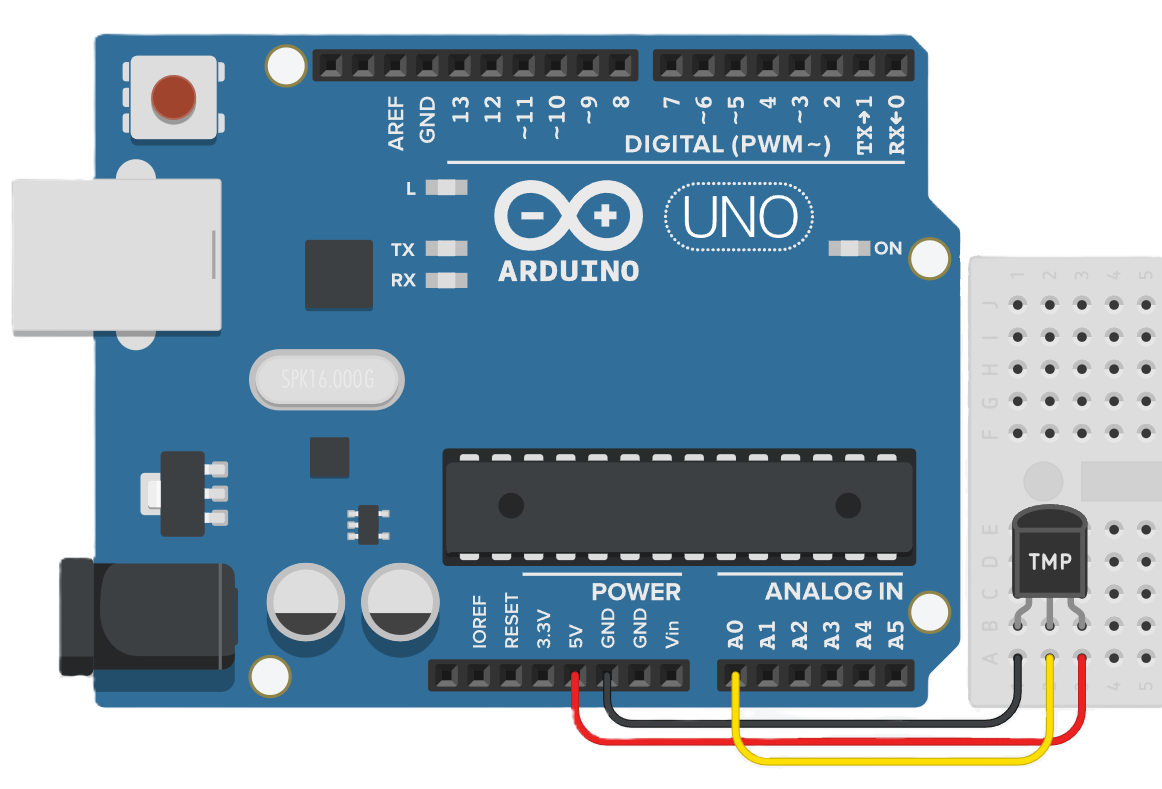
\includegraphics[width = \textwidth]{images/arduino/temp-pic.png}
                    \end{minipage}
                    \hfill
                    \begin{minipage}{0.49\textwidth}
                        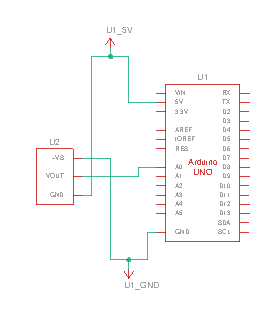
\includegraphics[width = \textwidth]{images/arduino/temp-scheme.pdf}
                    \end{minipage}
                    \caption{A sinistra una rappresentazione digitale del circuito realizzato per l'esperimento. A destra lo schema del circuito. Entrambe le illustrazioni sono state realizzate con Tinkercad\textsuperscript{\textregistered}.}
                    \label{fig:arduino-1}
            \end{figure}

            Per effettuare le misure ho usato il codice riportato di seguito. A intervalli di \SI{30}{\second} la lettura discreta di tensione data dal sensore\footnote{Come detto prima si tratta di un valore tra \num{0} e \num{1023}} e la converte in un numero decimale tra \SI{0}{\volt} e \SI{5}{V} attraverso la formula
            \begin{equation*}
                \frac{\text{\ttfamily (float)analogRead(SENSOR\_PIN)}}{\text{\ttfamily MAX\_READ}} * \text{\ttfamily MAX\_V}
                \mycomma
            \end{equation*}
            essendo $\text{\ttfamily MAX\_READ} = 1023$ e $\text{\ttfamily MAX\_V} = \SI{5}{\volt}$. Sapendo che a una tensione di \SI{0}{\volt} corrisponde una temperatura di \SI{0.5}{\celsius} e a \SI{4.5}{\volt} corrispondono \SI{100}{\celsius}, la conversione della lettura in gradi Celsius è data da
            \begin{equation}
                \bqty{\frac{\text{\ttfamily (float)analogRead(SENSOR\_PIN)}}{\text{\ttfamily MAX\_READ}} * \text{\ttfamily MAX\_V} - \text{\ttfamily A}} * \text{\ttfamily B}
                \mycomma
                \label{eq:arduino-temp-conv}
            \end{equation}
            dove $\text{\ttfamily A} = \SI{0.5}{\volt}$ e $\text{\ttfamily B} = \SI{100}{\celsius\per\volt}$ sono i fattori di scala.

            La conversione dei valori discreti in temperatura è eseguita dal codice tra le righe \texttt{23} e \texttt{26} applicando la \eqref{eq:arduino-temp-conv}. Vengono eseguite $\text{\ttfamily N} = 20$ misure consecuitive di cui è contestualmente calcolata la media che viene a sua volta stampata a schermo. Infine il codice attende il tempo mancante per raggiungere i \SI{30}{\second} dall'inizio del \txtloop.
            \lstinputlisting[language=C++]{code/arduino-temp.txt}
    \section{Dati}
        [aggiungere e commentare i dati]